\chapter{Sintesi di meccanismi}

\section{Introduzione}

Fino ad ora abbiamo affrontato problemi di analisi di meccanismi (analisi cinematica e analisi dinamica) che consistono in un problema in cui dato un sistema meccanico, si vuole studiare come funziona/le sue prestazioni.

tuttavia dal punto di vista ingegneristico più che ad analizzare il funzionamento di un meccanismo si è interessati a costruire un sistema che funzioni in un certo modo: si ha quindi il problema opposto.

In questo capitolo, di conseguenza, affronteremo il \textbf{problema della sintesi di meccanismi}. Lo stesso processo evolutivo degli esseri viventi può essere interpretato come un vastissimo problema di sintesi: ogni essere vivente ha cercato infatti di perfezionare se stesso, sia nel corpo che nelle capacità cognitive, in modo tale da sopravvivere.

Ci sono due aspetti nel problema di sintesi: 
\begin{enumerate}
\item Un aspetto matematico, ovvero quali sono i metodi matematici e numerici appropriati che mi consentono di risolvere un problema di sintesi.

Ci accorgeremo infatti che un problema di sintesi può essere formulato come un problema di \textbf{ottimizzazione}, che consiste nella ricerca di un massimo o di un minimo di una funzione.
\item Un aspetto ingegneristico, che consiste in come, dal problema fisico che sto cercando di risolvere, scrivo la funzione che voglio massimizzare o minimizzare.
\end{enumerate}

Per introdurre questo problema di sintesi viene proposto un esempio:

\begin{minipage}{.4\textwidth}
\centering
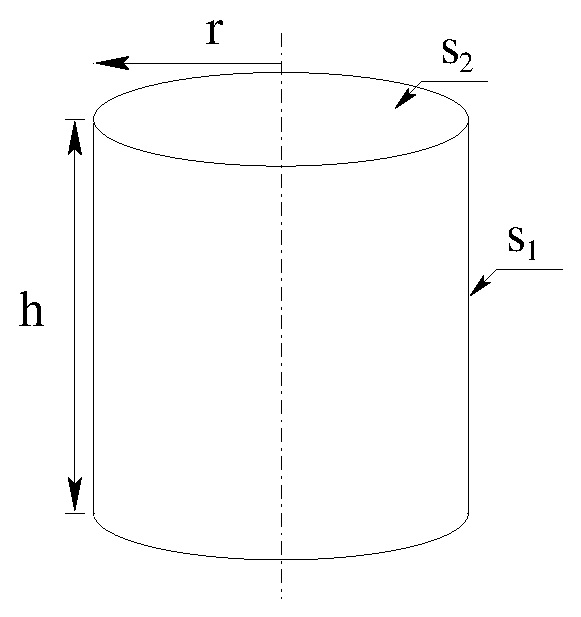
\includegraphics[width=.7\textwidth]{chapter08/immagine190}
\end{minipage}
\hfill
\begin{minipage}{.55\textwidth}
Immaginiamo di voler costruire un contenitore cilindrico che contenga un certo volume ($V_0$) e allo stesso tempo utilizzi il volume minimo di materiale.

Definiamo il raggio di base del cilindro (\emph{r}), la sua altezza (\emph{h}) e uno spessore delle superfici ($s_1$ per la superficie esterna, $s_2$ per le superfici di base).

Una volta nota la massa del materiale M e la sua densità ($\rho$), osseviamo che per minimizzare il volume del materiale si ha una certa libertà di scelta sulle grandezze \emph{h} e \emph{r}, e il problema di sintesi si può formulare nel seguente modo:
\end{minipage}

\[M = \rho\,(2\,\pi\,r\,h\,s_1\,+\,2\,\pi\,r^2\,s_2)\]
Trascurando lo spessore dei fondi, il volume del cilindro sarà dunque:
\[V = \pi\,r^2\,h\]
Si vuole a questo punto minimizzare il materiale (M(\emph{r},\emph{h})) agendo sulle grandezze (o \textbf{parametri di progetto}) \emph{r} e \emph{h}, soggetto alla condizione che $V = V_0$.

Il problema matematico che si è appena formulato è dunque un problema di minimizzazione vincolata.

Procediamo quindi a risolvere il problema di minimizzazione:
\begin{itemize}
\item La funzione da minimizzare risulta essere:
\[M(r,h) = 2\,\pi\,\rho\,(r\,h\,s_1\,+\,r^2\,s_2) = f(r,h)\]
\item  Il vincolo risulta essere:
\[g(r,h) = \pi\,r^2\,h\,-\,V_0\]
dove $V_0$ è un altro parametro	 che mi definisce la prestazione.
\end{itemize}

Al fine di risolvere un problema di minimizzazione vincolata, si può sfruttare il metodo di Lagrange: si procede dunque a definire una funzione di Lagrange
\[F(r,h, \lambda) = f(r, h) + \lambda\,g(r,h)\]
e si cerca il minimo di tale funzione.
\[
\begin{dcases}
\pd{F}{r} = 2\,\pi\,h\,r\,\lambda\,+\,\rho\,(2\,h\,\pi\,s_1\,+\,4\,\pi\,r\,s_2) = 0\\
\pd{F}{h} = \pi\,r^2\,\lambda\,+\,2\,\pi\,r\,s_1\,\rho = 0\\
\pd{F}{\lambda} = h\,\pi\,r^2\,-\,V_0 = 0
\end{dcases}
\]
Abbiamo ottenuto un sistema di 3 equazioni nelle incognite \emph{r},\emph{h} e $\lambda$, il quale, una volta risolto, permette di trovare i parametri che minimizzano la massa soggetta al vincolo (V - $V_ 0$).

Da un punto di vista ingegneristico, la massa M di un'ipotetica lattina è la \textbf{funzione obiettivo}, mentre la funzione V è il \textbf{vincolo}.

Immaginando a questo punto che gli spessori $s_1$ e $s_2$ non siano costanti qualsiasi ma dipendenti dai parametri di progetto (\emph{r} e \emph{h}): infatti più è alta la lattina, più lo spessore laterale deve essere maggiore; allo stesso modo più il raggio è maggiore, più lo spessore delle basi deve aumentare per evitare ingobbamenti del fondo (e in alcuni casi non sono piani, ma presentano curvature/corrugazioni); inoltre lungo la circonferenza di base è presente materiale di chiusura/cordone.

Possiamo dunque compiere una sintesi più completa scrivendo gli spessori come funzioni dei parametri di progetto e aggiungendo al calcolo della massa il cordone di fondo:
\[M = \rho\,(2\,pi\,r\,h\,s_1(r,h)\,+\,2\,\pi\,r^2\,s_2(r,h)\,+\,\text{cordone})\]
Questi aspetti trascendono l'aspetto matematico della sintesi di un meccanismo e sono riservati alla conoscenza dell'ingegnere.

Inoltre lo spessore delle pareti può non essere un numero reale, ma deve essere scelto fra una gamma finita di spessori predeterminati: il problema di ottimizzazione prevede che gli spessori siano valori discreti e non continui.

Possono essere aggiunti anche delle condizioni sui parametri di progetto in modo tale che, ad esempio:
\[h_{min} < h < h_{max}\qquad;\qquad r < r_{max}\]
In tale condizione sono presenti più funzioni di vincolo.

In altre parole, il problema di ottimizzazione consiste nel minimizzare una funzione soggetta a vincoli che possono essere sia delle uguaglianze che delle disequazioni. In alcuni casi il problema di ottimizzazione non viene formulato come un problema di minimizzazione, ma di massimizzazione: in tal caso se la funzione obiettivo deve essere minimizzata prende il nome di \textbf{funzione costo o penalità}, se la funzione obiettivo deve essere massimizzata prende il nome di \textbf{funzione merito o obiettivo}.

\section{Sintesi cinematica}

Ci focalizzeremo sulla sintesi cinematica di meccanismi: vedremo applicate le tecniche di ottimizzazione alla definizione delle dimensioni dei meccanismi al fine di ottenere particolari funzionalità.

Supponiamo che in un processo automatico di lavorazione si debba trasporare il corpo dalla posizione A alla posizione B con una contemporanea rotazione dello stesso di 90°. Si tratta di sintetizzare il sistema meccanico in grado di risolvere il problema proposto.

Si possono trovare molte soluzioni al problema in questione: si potrebbe avere un operatore umano o un robot che prende il corpo e lo sposta oppure si potrebbe avere un meccanismo che compie tale compito. Il meccanismo, ad esempio, potrebbe essere ideato in maniera tale da descrivere una traiettoria che prenda il corpo e lo trasporti nel punto B ruotandolo.
\begin{center}
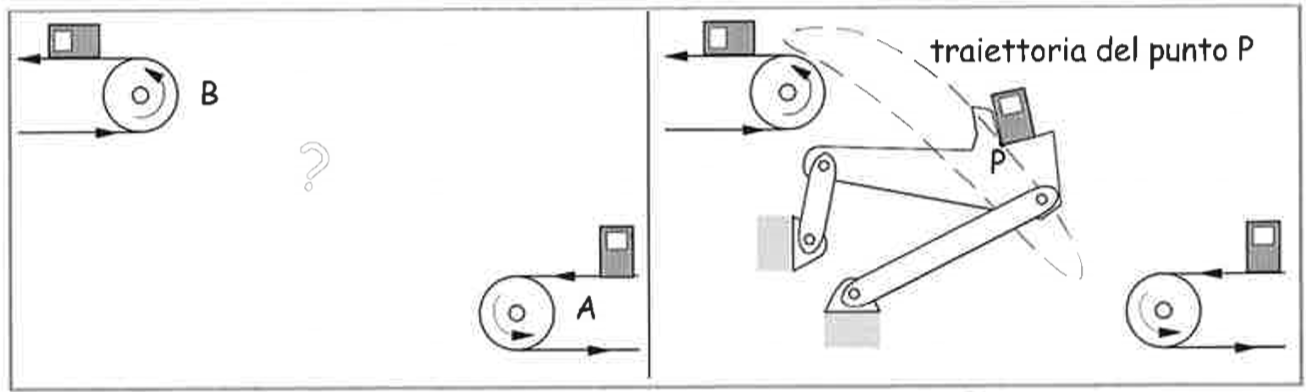
\includegraphics[width=.65\textwidth]{chapter08/immagine202}
\end{center}

Il vantaggio di quest'ultima soluzione rispetto alle altre è che il robot e l'uomo hanno bisogno di controllare il movimento e sono necessariamente più flessibili e più lenti: un meccanismo rigido, infatti, può raggiungere velocità che non possono essere raggiunte con un sistema controllato.

Quindi in altissima automazione può convenire realizzare delle macchine in cui è la forma geometrica delle stesse che realizza la funzione.
 
 È da precisare che sintetizzare non vuole dire inventare; l'operazione di sintesi consiste nell'utilizzo di una serie di procedure razionali per la scelta del tipo di sistema meccanico, del numero dei suoi membri ed infine delle sue dimensioni. Per tali motivi la sintesi viene convenzionalmente suddivisa in tre fasi:
 \begin{itemize}
 \item \emph{sintesi di tipo:} scelta del tipo di sistema meccanico (è stato scelto il sistema articolato piano);
 \item \emph{sintesi di numero:} definizione del sistema (il sistema articolato scelto è il quadrilatero, meccanismo composto da quattro membri collegati tra di loro da coppie rotoidali);
 \item \emph{sintesi dimensionale:} determinazione dele dimensioni degli organi del sistema
 \end{itemize}
 
 Un altro esempio di sintesi di una catena cinematica è la sospensione di una motocicletta. In realtà tale problema non è un problema di sintesi cinematica, bensì dinamica in quanto viene richiesto di progettare la sospensione della  motocicletta in modo tale che in funzione della corsa verticale della ruota la forza esercitata sul suolo abbia una certa caratteristica.
 
 Immaginiamo dunque di voler disegnare la sospensione di una motocicletta, prima ancora di decidere la lunghezza dei corpi o la rigideza delle molle si deve decidere come la ruota dovrà essere collegata a telaio (sintesi di tipo e di numero). Da questa sintesi si derivano diversi tipi di meccanismo con diverse caratteristiche di forza-spostamento verticale come rappresentato nella figura proposta:
 \begin{center}
 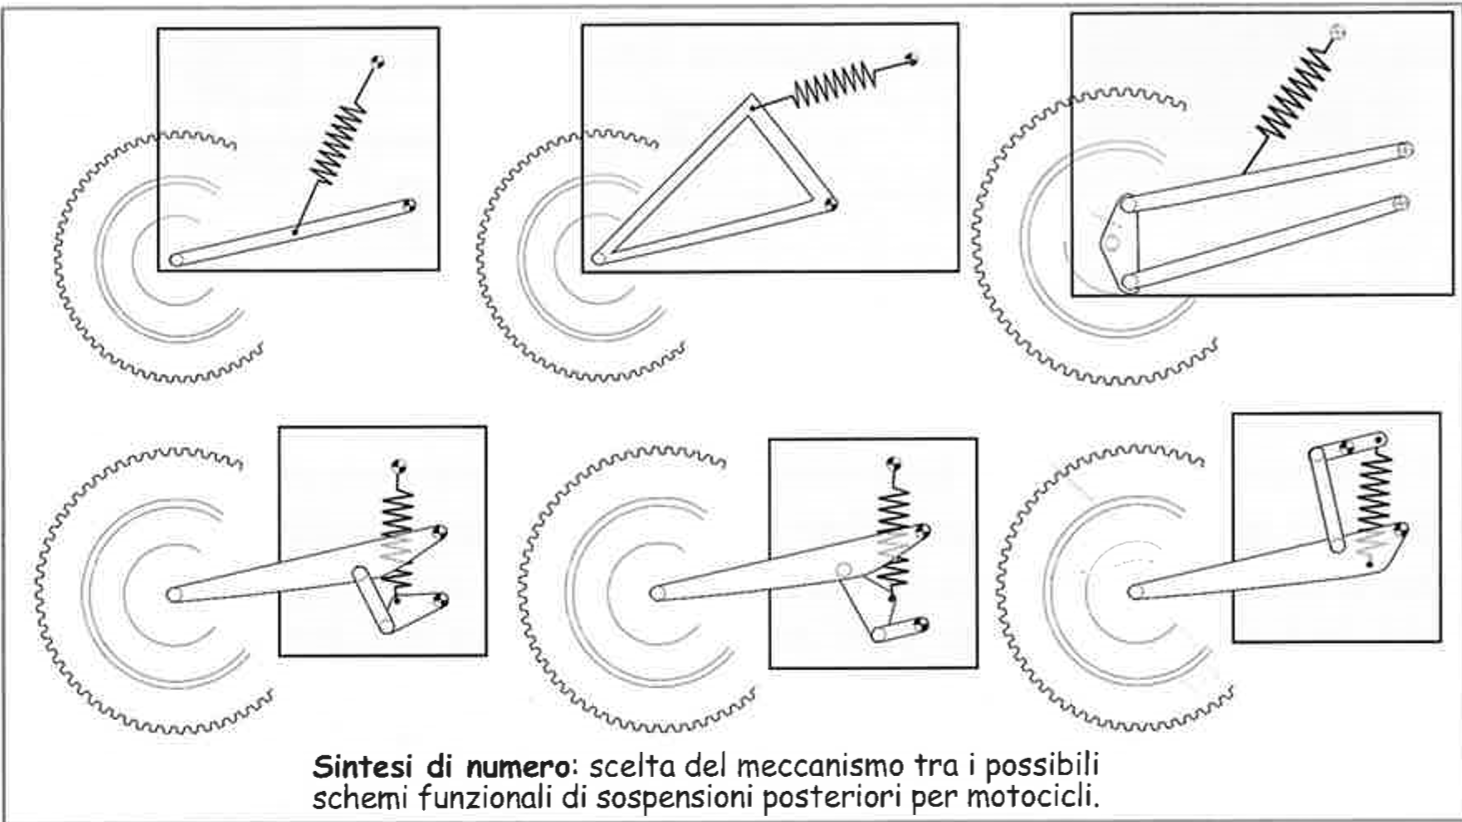
\includegraphics[width=.65\textwidth]{chapter08/immagine203}
 \end{center}
 
\subsection{Sintesi dei meccanismi articolati piani}

La sintesi si può distinguere in sintesi \textbf{strutturale} (di tipo e numero), che mira a stabilire il tipo di meccanismo, il numero dei suoi membri, la sua configurazione, i G.d.L. del meccanismo e in sintesi \textbf{dimensionale}, che ha il compito di determinare le dimensioni e le posizioni iniziali dei membri del meccanismo scelto.

Altresì, come diversi soo i compiti che un meccanismo è chiamato a svolgere, così pure si possono individuare problemi diversi che la sintesi cinematica deve risolvere, e cioè:
\begin{itemize}
\item problema della {\bfseries\emph{generazione di funzioni}} nel quale si richiede che il moto del membro condotto sia una funzione matematica del moto del membro motore;

Immaginiamo di avere un veicolo visto in pianta in cui le ruote posteriori non sono libere di sterzare. Al fine di poter curvare, dunque, sarà compito delle ruote anteriori di ruotare.

Nelle carrozze a cavalli le ruote erano collegate ad un unico assale/asse, il quale era collegato ai cavalli ed erano proprio quest'ultimi che permettevano la rotazione dell'assale in modo tale che durante la rotazione la carrozza ruotasse attorno ad un centro di istantanea rotazione individuato dall'intersezione dei prolungamenti dei due assi.

La soluzione con un assale unico tuttavia non risultava così prestante anche nei veicoli di fine `800, perché era l'uomo all'interno del veicolo che era responsabile di sterzare agendo sul volante.

Osserviamo dunque, dalla rappresentazione del veicolo in pianta che da un punto meramente cinematico il centro di istantanea rotazione dovrà trovarsi in uno dei punti sull'asse dell'assale posteriore, in quanto la velocità di avanzamento delle ruote è nella direzione del piano, di conseguenza il centro di istantanea rotazione si trova nella direzione ortogonale a tale piano.

\begin{center}
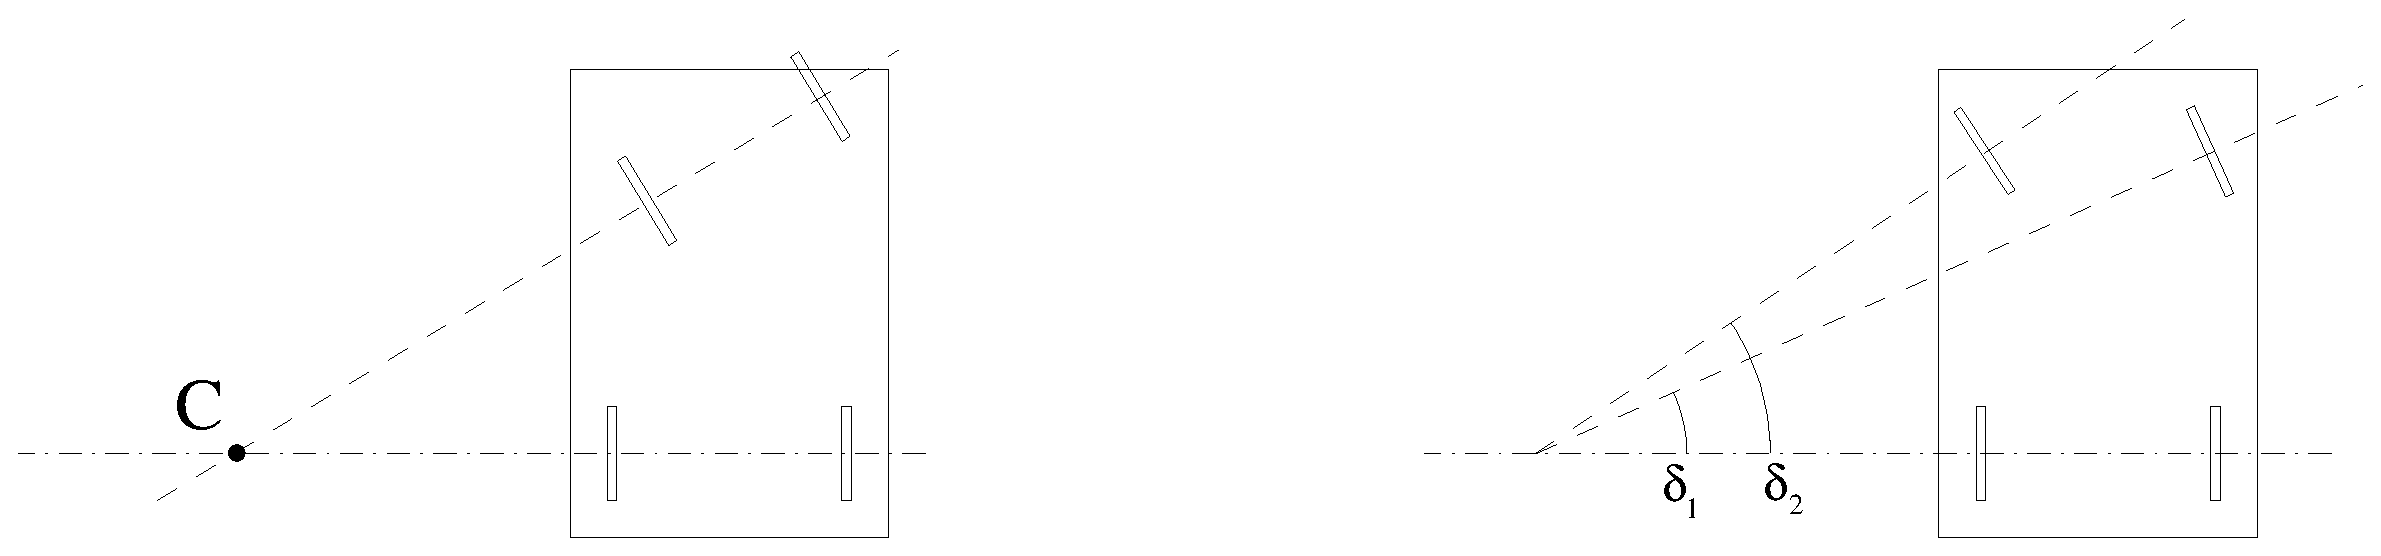
\includegraphics[width=.95\textwidth]{chapter08/immagine204}
\end{center}

L'angolo di sterzatura della ruota anteriore sinistra dovrà essere pari a $\delta_1$; la ruota anteriore destra, essendo più distante dal centro di istantanea rotazione dovrà, per conseguenza, girare di meno (di un angolo di sterzatura pari a $\delta_2$).

Sarà dunque necessario realizzare un meccanismo che, alla rotazione di un angolo $\delta$ del volante, permetta di realizzare, tramite due meccanismi, gli angoli di sterzatura richiesti dalle due ruote anteriori. In sostanza satà necessario ideare un  meccanismo che realizzi le funzioni: $f_1(\delta) = \delta_1 (\delta)$ e $f_2(\delta) = \delta_2 (\delta)$

È possibile soddisfare tali richieste si può realizzare con una catena cinematica (es. quadrilatero articolato) e la funzione che verrà realizzata lega il movente del meccanismo ad uno dei suoi cedenti per mezzo delle lunghezze dei suoi membri.

\item problema della {\bfseries \emph{generazione di traiettorie}}, nel quale si chiede che un punto vinolato ad un membro passi per determinati punti prefissati;

(cfr. gru per il sollevameto carichi aka Homework 1)
\item problema della {\bfseries \emph{guida di un corpo rigido}}, el quale si chiede che un corpo rigido passi per determinati punti con una prefissata orientazione;

Un esempio relativamente classico di tale problema è quello di una sospensione di un veicolo.

Si ha infatti un mozzo della ruota (assunto corpo rigido) e si vuole che la ruota si muova secondo una certa traiettoria in particolare a mano a mano che le sospensioni funzionano si vuole che il veicolo si inclini lateralmente sulle curve e che quindi la sospensione interna si abbassi e quella esterna si allunghi, mantenendo la ruota il più ortogonale possibile al suolo.

Per realizzare tale funzione si utilizza, molto frequentemente, una sospensione a doppio braccio oscillante. Altre categorie di sospensioni riguardano l'utilizzo di una guida prismatica (cfr. sospensione Mc. Pherson).

In sostanza le sospensioni dei veicoli rientrano nella categorie di guida dei corpi rigidi proprio perché il loro compito è quello di controllare l'orientazione e la traiettoria della ruota rispetto alla carrozzeria.
\end{itemize}

Fino a 20 anni fa il problema di sintesi veniva risolto tramite tecniche per punti di precisione, (ora vengono utilizzate tecniche di ottimizzazione): esse consistono nel risolvere la catena cinematica in un certo numero di posizioni e imporre che la lunghezza delle aste sia tale per cui il punto o la funzione che io desidero raggiungere/realizzare sia reallizzata nei punti discretti in cui si va a risolvere il meccanismo.

In altre parole consiste, nella generazione di traiettoria, nell'imporre che il punto E della gru passi per un certo numero di punti. Il numero di punti di precisione che si possono imporre è, tuttavia, generalmente molto piccolo (in tali condizioni il comportamento della traiettoria tra i punti di precisione è difficilmente controllabile).

\subsection{Sintesi dimensionale con tecniche di ottimizzazione}

Si immagini di voler costruire un quadrilatero articolato in gradi di generare la funzione $\gamma = \gamma(\alpha)$ dove $\alpha$ e $\gamma$ sono rispettivamente la rotazione della manovella motrice e la rotazione della manovella condotta.

Se sono state assegnate le posizione dei perni di manovella, i parametri di progetto, su cui si può agire per ottenere le caratteristiche desiderate, in questo caso sono: le lunghezze $h_1, h_2, h_3$ dei membri, la rotazione $h_4$ della manovella motrice nella condizione iniziale.

Se si assegnano dei valori arbitrari ad $h_1, h_2, h_3$ ed a $h_4$ si ottiene un meccanismo in grado di generare una funzione $f(\alpha)$ diversa dalla funzione desiderata $\gamma(\alpha)$; la  differenza $e(\alpha) = f(\alpha) - \gamma(\alpha)$, chamata errore strutturale, dipende solo dai parametri di progetto $h_1, h_2, h_3$ ed $h_4$. Questa osservazione è alla base del metodo di sintesi con tecniche di ottimizzazione; infatti è possibile costruire una funzione penalità legata all'errore strutturale e cercare i valori dei parametri di progetto $h_1, h_2, h_3$ ed $h_4$ in grado di minimizzare tale funzione e quindi  l'errore strutturale del meccanismo.

La minimizzazione viene effettuata in maniera automatica, partendo da un meccanismo di primo tentativo, con delle opportune ruotine che possono usare algoritmi di ricerca di tipo derivativo o non derivativo.
\begin{center}
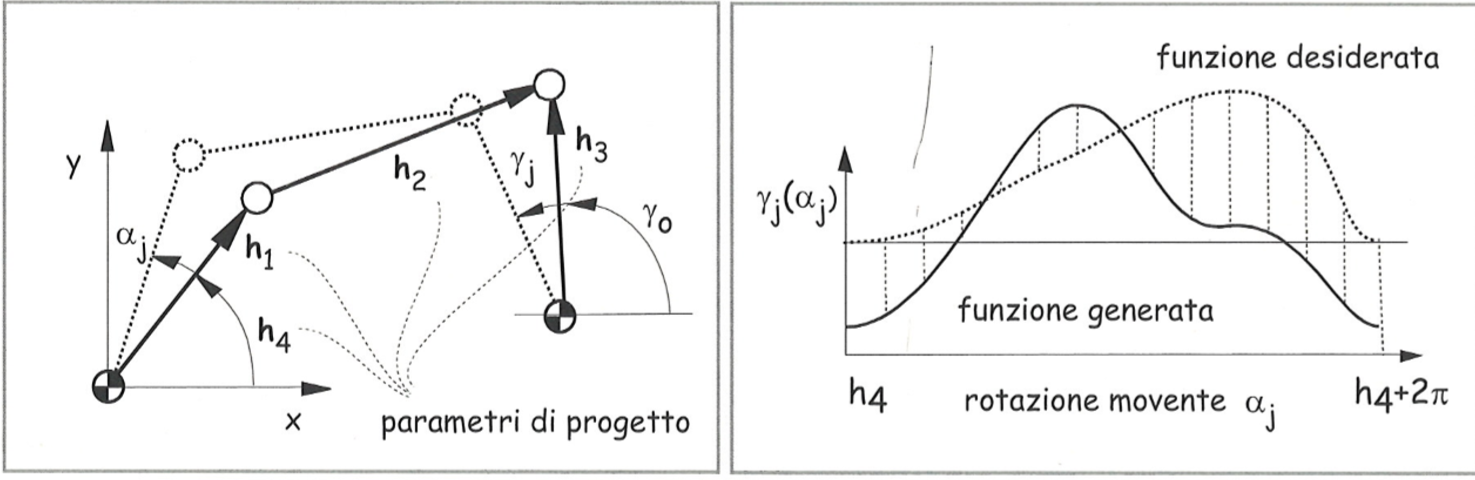
\includegraphics[width=.75\textwidth]{chapter08/immagine205}
\end{center}

Vale la pena porre in luce che con questo tipo di sintesi non si ottiene un meccanismo in grado di annullare l'errore strutturale in alcuni punti, ma un meccanismo ``ottimo'' che rende minimo (\emph{ma non annulla}) l'errore strutturale in tutto il camo di movimento del meccanismo.

Il metodo può essere esteso a meccanismi più complessi con un maggior numero di parametri di progetto e può essere utilizzato anche per la sintesi di meccanismi di traiettoria o di moto rigido.

\begin{center}
{\scshape{\bfseries Sintesi ottimale di un quadrilatero generatore di una traiettoria a forma concoidale}}
\end{center}

Un esempio di sintesi ottimale di un meccanismo generatore di traiettoria è riportato in figura. In essa sono disegnati il meccanismo con i parametri di progetto e la traiettoria desiderata (\emph{una concoide}), mentre nella tabella sono raccolti i parametri del meccanismo di primo tentativo, i parametri del meccasnimo ottimizzato ed i campi di variabilità dei parametri di progetto, che, come si può osservare, in questo caso sono molto ampi.
\begin{center}
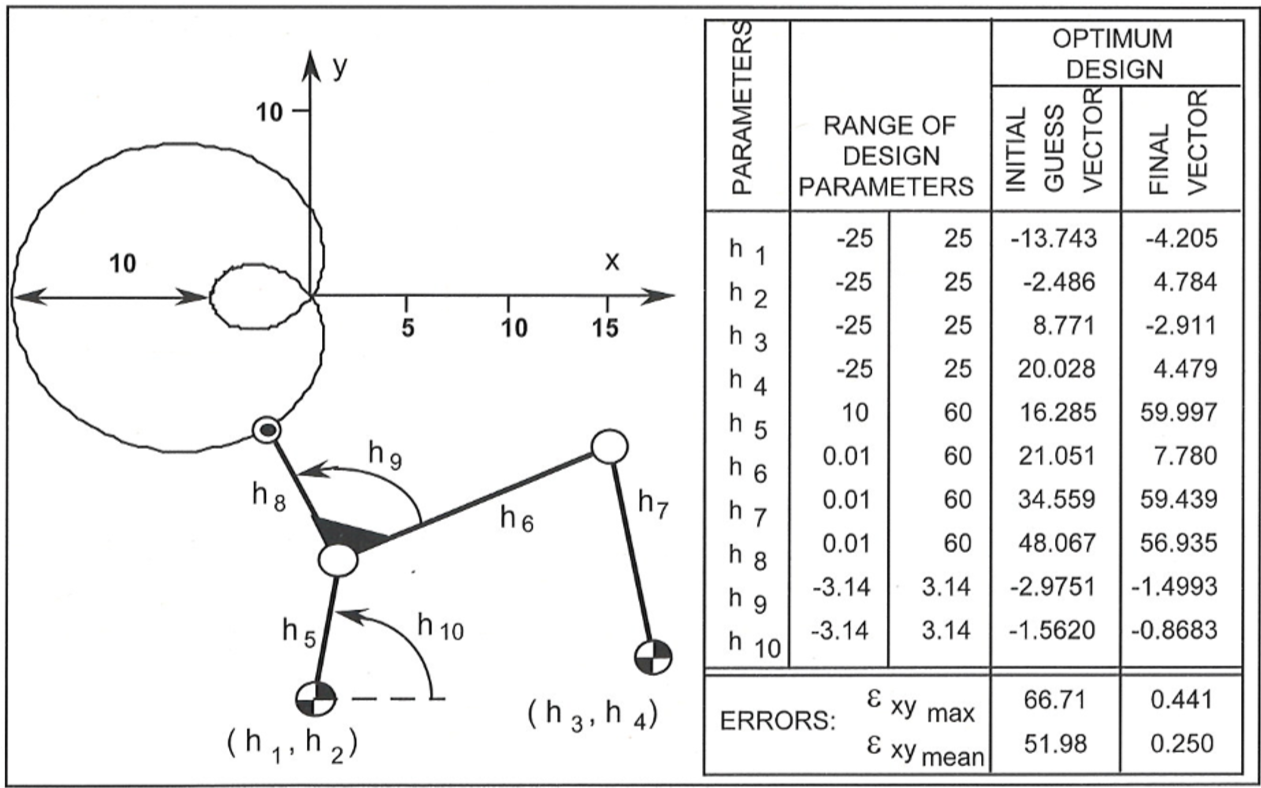
\includegraphics[width=.45\textwidth]{chapter08/immagine206}
\end{center}

La tabella mostra anche la drastica riduzione dell'errore strutturale (\emph{errore tra traiettoria ottenuta e desiderata}) che si è conseguita tramite il processo di ottimizzazione; a conferma di questo dato nella figura seguente sono rappresentate le traiettorie generate dal meccanismo di primo tentativo e dal meccanismo ``ottimo''.
\begin{center}
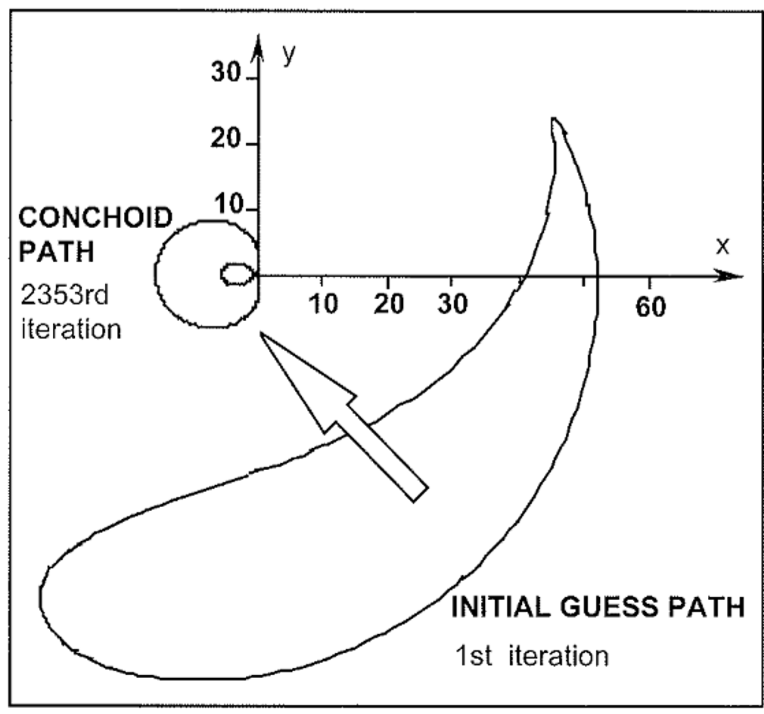
\includegraphics[width=.35\textwidth]{chapter08/immagine207}
\end{center}

\section{Sintesi di un meccanismo generatore di traiettoria}

Entriamo più nel concreto della sintesi cinematica e vediamo il caso della sintesi di un meccanismo generatore di traiettoria, in seguito vedremo come adattare questo problema ad altri tipi di sintesi.

Abbiamo detto che la sintesi consiste nel risolvere un problema di ottimizzazione: lo scopo principale sarà dunque la minimizzazione (o massimizzazione) di una funzione.

Sarà dunque necessario convertire, in qualche maniera, il nostro problema ingegeristico in un problema matematico di minimizzazione; si dovrà di conseguenza scrivere una funzione \emph{f} di un numero arbitrario di parametri (\emph{f} = \emph{f}($P_1, \dots, P_N$)) che rappresenti il valore della nostra soluzione o una penalità (distanza della funzione da quella ideale) che dipenda dai parametri di progetto sui quali è possibile agire/cambiare.

Tale minimizzazione della funzione \emph{f} sul vettore dei parametri di progetto \textbf{P} è vincolata da funzioni del tipo:
\[g(\mathbf{P}) = 0 \qquad\lor\qquad h(\mathbf{P}) < 0\]
Il compito dell'ingegnere è quello di convertire il problema ingegneristico in uno matematico e dare un'espressione alle funzioni \emph{f}, \emph{g} e \emph{h}.

Per fare ciò sarà opportuno  eseguire in primo luogo una sintesi di numero e tipo, che, in altre parole, consiste nell'individuare le varibili su cui possiamo agire nella catena cinematica (\textbf{P} = $P_1, \dots, P_N$).

Affrontiamo tale argomento eseguendo la sintesi del sistema di sterzo.
\subsection{Sintesi di un meccanismo di sterzo}

\begin{minipage}{.5\textwidth}
Immaginiamo di avere una ruota anteriore solidale ad una manovella (tirante dello sterzo): in questo modo la ruota può ruotare attorno all'asse di sterzatura che è mosso dal tirante.

Il tirante sarà collegato ad un corpo intermedio la cui rotazione è controllata dal volante e il sistema si ripeterà simmetrico anche per la rimanente ruota anteriore. 

Ad una rotazione $\delta$ del corpo centrale (aka sterzo), seguirà una rotazione $\delta_1$ della ruota di sinistra e una rotazione $\delta_2$ della ruota di destra.
\end{minipage}
\hfill
\begin{minipage}{.5\textwidth}
\centering
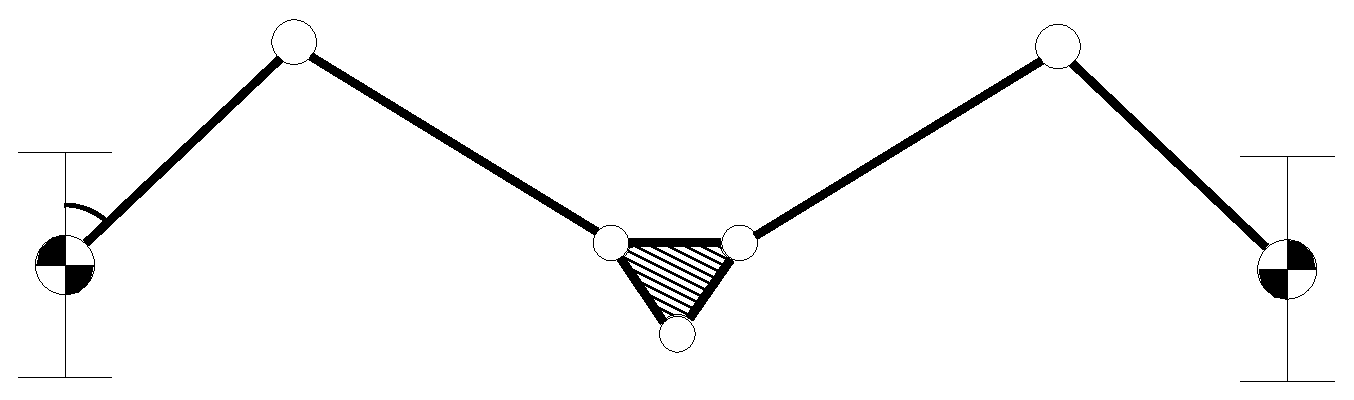
\includegraphics[width=.75\textwidth]{chapter08/immagine208}
\end{minipage}

Così facendo è stato implicitamente scelto che la catena cinematica generatrice di funzione è un quadrilatero (in realtà nell'insieme è un esalatero, tuttavia posso immaginare due quadrilateri separati responsabile della sterzatura delle due ruote).

\begin{minipage}{.5\textwidth}
\centering
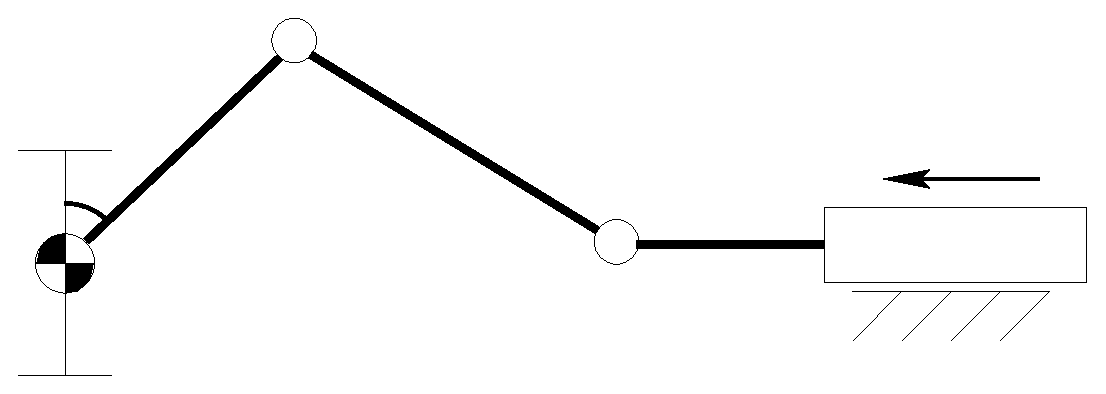
\includegraphics[width=.75\textwidth]{chapter08/immagine209}
\end{minipage}
\hfill
\begin{minipage}{.5\textwidth}
Questa non è l'unica soluzione possibile per realizzare un meccanismo di sterzo: avrei potuto, infatti, avere comunque il tirante dello sterzo incernierato a telaio e, al posto di un meccanismo RRRR, un meccanismo RRRP, nel quale lo spostamento del pistone spinge la biella che, a sua volta, permette la rotazione della ruota ({\bfseries \emph{meccanismo di sterzo a cremagliera}}: il volante fa girare la ruota dentata che spinge la cremagliera a destra o a sinistra).
\end{minipage}

Una volta eseguita la sintesi di numero e tipo sarà possibile, tramite un'analisi cinematica del meccanismo scelto, ricavare l'angolo $\delta_1$ come funzione del'angolo di sterzo ($\delta$) e delle lunghezze dei membri del meccanismo stesso ($P_1, \dots , P_N$).
\[\delta_1 = f(\delta, P_1, \dots, P_N)\]
In altre parole tramite l'analisi cinematica si è trovata un'espressione matematica tra il cedente ($\delta_1$) come espressione dei parametri di progetto (\textbf{P}) e del movente/coordinata libera ($q = \delta$).

La funzione \emph{f} prende il nome di \textbf{funzione realizzata}.

Come faccio a sapere se i parametri di progetto di primo tentativo (\textbf{P}) sono adeguate per la funzione che si vuole realizzare?

Al fine di capire se i parametri di progetto sono appropriati per la realizzazione della funzione, si introduce una nuova funzione $f_d$ che prende il nome di \textbf{funzione desiderata}.

\begin{center}
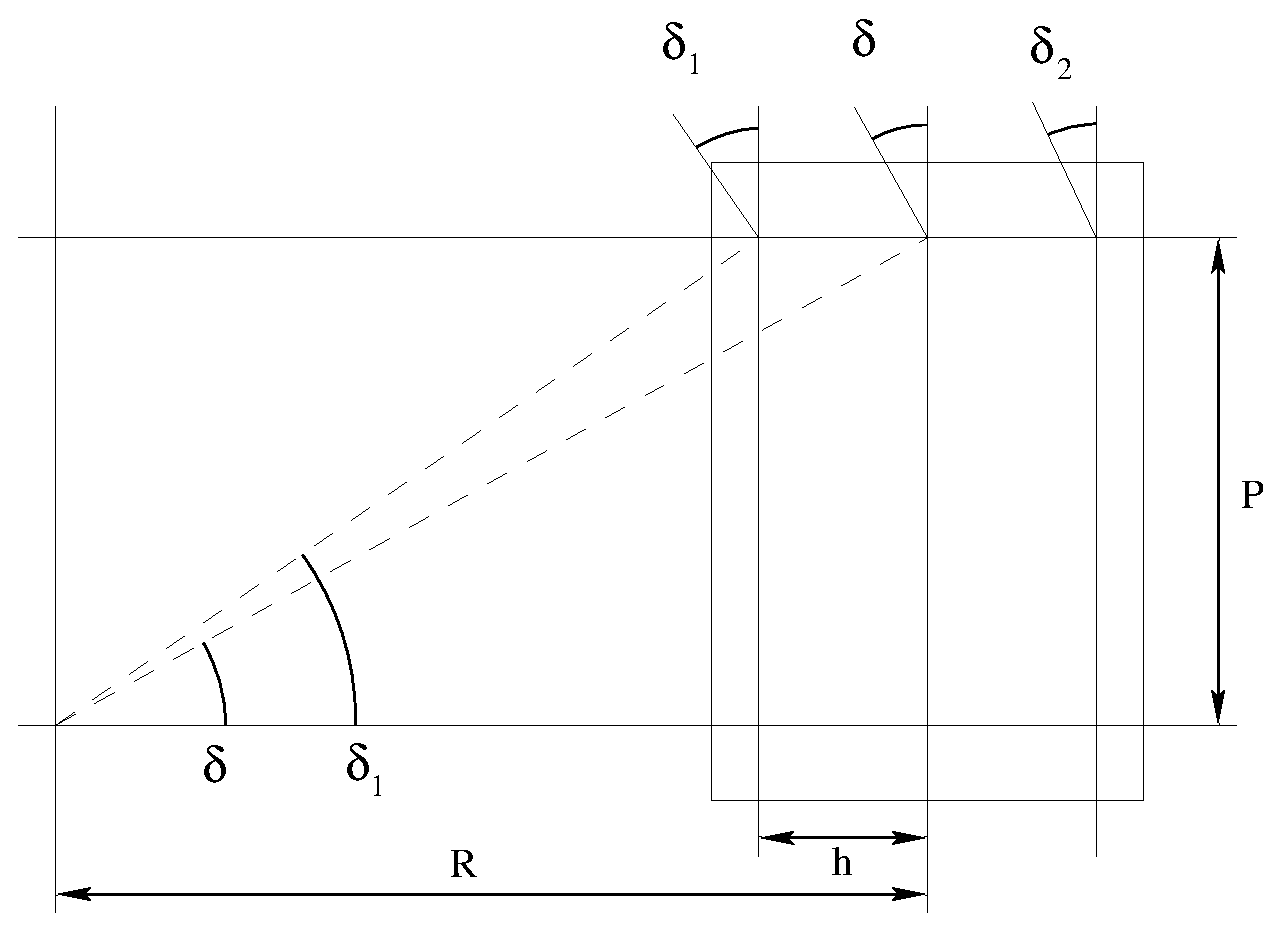
\includegraphics[width=.75\textwidth]{chapter08/immagine210}
\end{center}
Vediamo come applicare tutti gli strumenti fino ad ora acquisiti per formulare un espressione di una funzione che leghi l'angolo di sterzata delle due ruote con quella del volante (cfr. problema di Ackermann o della sterzatura cinematica).

Consideriamo una vista in pianta di un veicolo nell'atto di sterzatura attorno ad un centro di istantanea rotazione (appartenente al prolungamento dell'asse posteriore) e definiamo alcune grandezze:
\begin{itemize}
\item Sia C il generico centro di istantanea rotazione del veicolo in fase di sterzata;
\item Sia R il raggio di curvatura del veicolo riferito all'assale posteriore;
\item Sa P il passo del veicolo, ovvero la distanza tra l'asse delle ruote posteriori e l'asse delle ruote anteriori
\item Sia h la metà della careggiata anteriore
\end{itemize}
Sotto tali ipotesi possiamo osservare che il mozzo della ruota anteriore sinistra in fase di sterzata dovrà convergere nel centro di istantanea rotazione, descrivendo un angolo pari a $\delta_1$ (coincidente con l'angolo che la ruota dovrà sterzare).

La manovella che muove la biella anteriore è supposta incernierata nel centro dell'asse anteriore, essa desciverà un angolo $\delta$ che corrisponde all'angolo di sterzatura cinematica (è un angolo fittizio che corrisponde sostanzialmente, a meno del rapporto di moltiplicazione del volante, con l'angolo di sterzatura del volante). 

Analogamente alla ruota interna anche la ruota esterna seguirà lo stesso principio e descriverà un angolo $\delta_ 2$.

Alla luce delle considerazioni fatte durante la sintesi di tipo e numero, si è in grado di determinare l'angolo di rotazione delle due ruote dalla conoscenza dell'angolo di sterzatura in modo che i mozzi delle ruote in esame convergano verso il centro di istantanea rotazione.

Infatti, noto che:
\[\tan{\delta} = \cfrac{P}{R}\qquad;\qquad \tan{\delta_1} = \cfrac{P}{R\,-\,h}\qquad;\qquad\tan{\delta_2} = \cfrac{P}{R\,+\,h }\]
È possibile ricavare il raggio di curvatura dalla prima equazione e, sostituendole alle rimanenti due equazioni, ricavare gli angoli di rotazione delle ruote anteriori.

Per semplificare ulteriormente i relativi calcoli, tuttavia, si preferisce utilizzare la \textbf{curvatura} al posto del raggio di curvatura. Infatti per $\delta = 0$ la prima equazioni è verificata se e solo se $R\,\to\,\infty$. Sia dunque la curvatura:
\[\theta = \cfrac{1}{R}\]
In questo modo è stata introdotta una grandezza continua che permettere di distinguere i casi in cui il veicolo stia sterzando a destra o a sinistra.

Così facendo:
\[
\begin{dcases}
\tan{\delta} = P\,\theta\\
\tan{\delta_1} = \cfrac{P}{R-h} = \cfrac{P}{\cfrac{1}{\theta}\,-\,h} = \cfrac{\theta\,P}{1\,-\,h\,\theta} = \cfrac{\theta\,P}{1\,-\,\cfrac{h}{P}\,\theta\,P}
\end{dcases}
\]
In questo modo ho ricavato l'espressione:
\[\tan{\delta_1} = \cfrac{\tan{\delta}}{1\,-\,\cfrac{h}{P}\,\tan{\delta}}\qquad\iff\qquad \delta_1 = \arctan{\cfrac{\tan{\delta}}{1\,-\,\cfrac{h}{P}\,\tan{\delta}}}\]

Un ragionamento analogo può essere realizzato per l'angolo $\delta_2$, ottenendo:
\[\delta_2 = \arctan{\cfrac{\tan{\delta}}{1\,+\,\cfrac{h}{P}\,\tan{\delta}}}\]

Abbiamo così ottenuto le due funzioni desiderata per la realizzazione della sterzatura del veicolo.

Ora dobbiamo determinare le funzioni determinare le funzioni realizzate che è strettamente dipendente dal meccanismo scelto nella sintesi di tipo e numero.

Nel quadrilatero rappresentato possiamo riconoscere ben 6 parametri di progetto per la realizzazione della funzione realizzata ($\alpha, L_1, L_2, L_3, L_4, \beta$);

\begin{minipage}{.5\textwidth}
 a questo punto muovendo di una certa quantità l'angolo $\delta$ dovrò calcolare l'angolo $\delta_1$ che si realizza effettivamente: per far ciò eseguo l'analisi cinematica del quadrilatero.

sia dunque \emph{F} la funzione per cui è possibile ricavare l'angolo $\delta_1$, dipedente da $\delta$ e dai parametri di progetto:
\[\delta_1 = F(\delta, \alpha, L_1, L_2, L_3, L_4, \beta)\]
\end{minipage}
\hfill
\begin{minipage}{.5\textwidth}
\centering
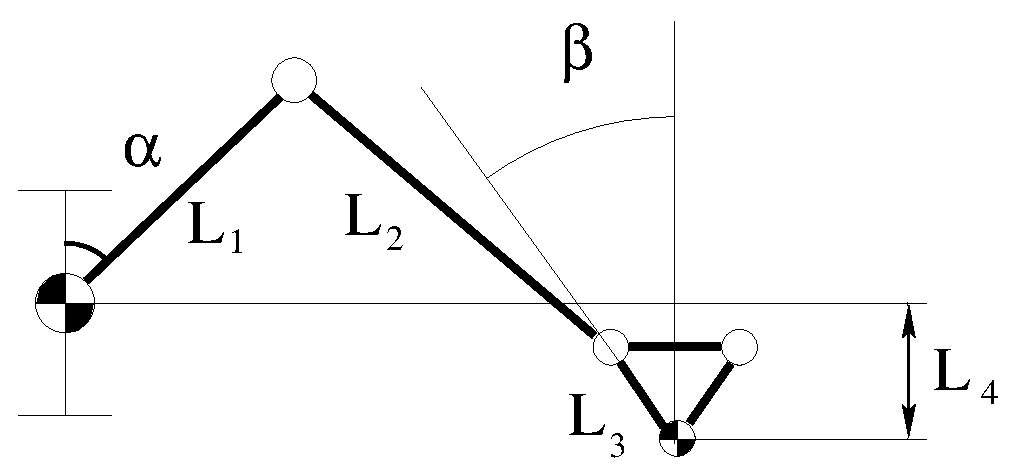
\includegraphics[width=.8\textwidth]{chapter08/immagine211}
\end{minipage}
\vspace{1mm}

A questo punto, per poter riscrivere il problema di sintesi come un problema di ottimizzazione si può definire una nuova funzione, da minimizzare, detta \textbf{funzione errore}
\[\epsilon = \text{Funzione desiderata} \, -\,\text{Funzione realizzata} = \epsilon(\delta, \mathbf{P})\]

\section{Impostazione del problema di ottimizzazione}

Abbiamo visto che risolvere un problema di sintesi significa produrre un sistema meccanico in modo tale che realizzi una funzione desiderata. In particolare si è esplicitato il nostro interesse nei confronti della sintesi cinematica di meccanismi che rispettino una ben precisa funzionalità cinematica.

Abbiamo inoltre visto che ci possono essere tre tipi di funzionalità realizzabili: generazione di funzione, generazione di traiettoria e generazione di moto rigido.

In ogni caso si dovrà sempre specificare:
\begin{enumerate}
\item Il tipo di catena cinematica
\item Il numero dei parametri di progetto
\item La funzione desiderata (in funzione del movente): ricavata dalla specifica del problema che si desidera risolvere
\item La funzione realizzata: ricavata dall'analisi cinematica del meccanismo definito nella sintesi di tipo e numero del meccanismo
\item La funzione errore da minimizzare nel problema di ottimizzazione (differenza tra funzione desiderata e funzione realizzata) 
\end{enumerate}

Così facendo abbiamo espresso il problema di sintesi come un problema di ottimizzazione: infatti, il fatto che la funzione desiderata sia solo funzione del movente e che la funzione realizzata sia anche funzione dei parametri di progetto, permette di, agendo sui parametri di progetto, minimizzare la distanza/differenza tra le due, la quale è espressa dalla funzione errore.

Non a caso è stato utilizzato il termine distanza: tale termine, difatti, è stato già introdotto nei corsi di Analisi quando si è trattata la \textbf{convergenza uniforme}.

Immaginando di rappresentare in un grafico le due funzioni in esame (realizzata e desiderata) in un intervallo di valori del movente (es. $\delta$).
Esistono vari metodi per la quantificazione della distanza tra due curve/funzioni:
\begin{enumerate}[$\rightarrow$]
\item Per ogni valore di $\delta$ si può procederà al calcolo dell'estremo superiore, definito come:
\[\epsilon^*(\mathbf{P}) = \text{sup}_{\delta}(\norma{F_D\,-\,F_R})\]
(la diversa notazione di $\epsilon$ è stata scelta per distinguerla dalla distanza puntuale $\epsilon(\delta, \mathbf{P})$)

Il significato matematico di tale espressione della distanza permette di quantificare la massima differenza tra le due funzioni, che potrà essere sfruttata come metro/criterio di distanza tra le due curve.

Se dunque la distanza massima tende a zero, si avrà quello che in gergo è definita come convergenza uniforme.

Tuttavia questo metodo non è l'unico per il calcolo della distanza, e non risulta essere molto comodo per la risoluzione del problema di ottimizzazione in quanto non tiene in cosiderazione la distanza media tra le due curve: ad esempio potrebbe presetarsi il caso in cui la distanza massima fosse elevata in uno degli estremi dell'intervallo di $\delta$, ma che mediamente la differenza tra le due curve fosse molto bassa.

La modalità di calcolo della distanza proposta prende il nome di \textbf{norma infinito} e viene anche indicata tramite la notazione:
\[\epsilon^*(\mathbf{P}) = \norma{F_D\,-\,F_R}_{\infty}\]
\item Si potrebbe dunque pensare di utilizzare come metro di giudizio la distanza media tra le due curve:
\[\epsilon^* = \cfrac{1}{\delta_{max}\,-\,\delta_{min}}\,\int_{\delta_min}^{\delta_{max}}\,\norma{\epsilon(\delta,\,\mathbf{P})}\,d\delta\]
In questo modo, punto per punto, si sta calcolando la distanza tra le due funzioni, se ne sta prendendo il valore assoluto e si sta calcolando il valore medio della distanza sull'dominio della funzione errore puntuale.

Questo calcolo permette di determinare quanto diverse siano le due funzioni in media.

La modalità di calcolo della distanza proposta prende il nome di \textbf{norma L1} e viene anche espressa tramite la notazione:
\[\epsilon^* =\norma{F_D\,-\,F_R}_1\]
\item In alternativa alla norma L1 riconosciamo l'esistenza della \textbf{norma quadratica} o \textbf{norma L2}.

Potrei infatti definire la distanza tra le due funzioni come:
\[\epsilon^* = \norma{F_D\,-\,F_R}_2 = \cfrac{1}{\delta_{max}\,-\,\delta_{min}}\,\int_{\delta_{min}}^{\delta_{max}}\,(F_D\,-\,F_R)^2\,d\delta\]
Eseguendo l'integrale del quadrato dell'errore puntuale tendo ad annullare l'errore in media, ma tendo a dare un po' più importanza ai punti che presentano una errore puntuale elevato.

Infatti è possibile interpretare la norma L2 come l'errore tra le due curve pesato proporzionalmente all'errore stesso.

La quantità appena definita è in gergo definita con il nome di \textbf{errore quadratico medio} o \textbf{root mean squared} ($\epsilon_{RMS}$).

Il limite di quest'ultimo approccio risiede nella difficoltà di calcolo dell'integrale ed è computazionalmente molto complicato. È tuttavia possibile approssimare l'integrale con una sommatoria.

Si procede a dividere il dominio delle due curve in N punti $\delta_i$ (detti \textbf{punti di accuratezza}), si calcolano i valori delle due funzioni i suddetti punti e al posto di eseguire l'integrale si esprime la norma L2 come:
\[\epsilon^* = \cfrac{1}{N}\,\sum_i\,(F_{Di}\,-\,F_{Ri})^2\]
\end{enumerate}

\section{Approfondimento sui metodi di ottimizzazione}

Per comprendere e cotrollare il processo di minimizzazione della funzione penalità risulta necessario capire come funzionano le tecniche di ottimizzazione: su questo argomento esistono interi corsi di studio però un conto è affrontare il problema da un punto di vista matematico o di algoritmi, un altro è quello di formulare un problema di ottimizzazione.

Esistono due grandi categorie per la determinazione di massimi e minimi di una funzione: la ricerca dei minimi globali (che si effettua in Wolfram Mathematica tramite la funzione NMinimize/NMaximize) o la ricerca dei minimi locali.

Inoltre la ricerca dei minimi può essere sia \textbf{vincolata} che \textbf{non vincolata}: ovvero se al problema di sintesi/ottimizzazione sono presenti o meno uguaglianze o disuguaglianze applicate sui parametri di dipendenza della funzione penalità.

Il metodo di Lagrange, ad esempio, permette di trasformare una minimizzazione vincolata con uguaglianza in una minimizzazione non vincolata. A testimonianza che è possibile trasformare un problema di ricerca dei minimi vincolata in una non vincolata in quanto gli algoritmi (metodi numerici per la risoluzione del problema) per risolvere la prima tipologia sono diversi da quelli per risolvere la seconda tipologia di problema.

Un altro modo per convertire un problema di minimizzazione vincolata in uno di minimizzazione non vincolata è il cosiddetto \textbf{approccio di penalità}: la minimizzazione di una funzione \emph{f(\textbf{x})} soggetta a vincoli può essere trattata come una ricerca dei minimi non vincolata della funzione:
\[f(\mathbf{x})\,+\,\omega_1\,g(x)^2\,+\,\omega_2\,h^+(\mathbf{x})^2\]
dove:
\begin{itemize}
\item \emph{f(\textbf{x})} è la funzione da minimizzare
\item \emph{g(\textbf{x})} è il vincolo espresso come uguaglianza
\item \emph{h(\textbf{x})} è il vincolo espresso come disuguaglianza (in questo esempio il vincolo è h < 0)
\item $h^+$(\textbf{x}) è la parte positiva del vincolo espresso come disuguaglianza
\item $\omega_1$ e $\omega_2$ sono i pesi che quantificano l'influenza dei vincoli nel processo di minimizzazione (tanto più sono alti i pesi quanto i vincoli moltiplicati saranno influenti).

Quanto sono disposto a tollerare la violazione di un vincolo?
\end{itemize}

In questo modo, riformulando la funzione penalità, anche se si raggiungesse un valore per cui \emph{f(\textbf{x})} fosse minima, ma fosse stato violato un vincolo, la funzione penalità  risentirebbe di tale violazione aggiungendo un termine quadratico.

Da un punto di vista ingegneristico si è interessati a determinare il maggior numero possibile di punti minimi locali in quanto ad ognuno di essi corrisponde una configurazione diversa del meccanismo, a soluzioni ingegneristiche diverse e ad un range maggiore di possibilità di configurazione del meccanismo tra cui scegliere (anche alla luce di considerazioni geometriche / d'ingombro).

Gli algoritmi che trattano l'ottimizzazione/minimizzazione vincolata e non vincolata appartengono a due grandi tipologie: \textbf{NMinimize} che contiene diversi metodi per la minimizzazione vincolata e \textbf{FindMinimum} che contiene algoritmi di minimizzazione non vincolata.